\label{chap:literature}
TODO: write intro here, mentioning the main themes:

Similarity

\gls{propaganda}

Propaganda and misinformation

\Gls{political-leaning}: definitions/classification


\section{Persuasion}
\label{sec:lit_persuasion}

Persuasion definition~\cite{gass2018persuasion}: \gls{persuasion} can influence a person's beliefs, attitudes, intentions, motivations, or behaviours.
Umbrella term for many forms: \gls{propaganda} (to indoctrinate a population towards an individual or a particular agenda), sentiment, \gls{populism}, coercion (aggressive threats and the provocation of fear and/or shame to influence a person's behavior.)

\subsection{Propaganda}
\label{sec:lit_propaganda}
TODO propaganda definition in different fields.

First of all, let us start with a definition of propaganda.
We can define propaganda as the use of language ``with the intention of influencing people's opinions."\footnote{\url{https://dictionary.cambridge.org/dictionary/english/propaganda}}
It has many points in common with argumentation/rhetorics and is usually associated with deceiving techniques, partial point of views, logical fallacies.
In his book on propaganda, Edward Bernays defines it as a ``consistent, enduring effort to create or shape events to influence the relations of the public to an enterprise, idea or group''~\cite{bernays}.

Propaganda has a set of distinctive features beyond its persuasive function. It usually has a sizable target audience, it represents a specific group's agenda, and makes use of faulty reasoning and/or emotional appeals~\cite{miller1939techniques}.

Injecting propaganda in the political narrative is an old and common tactic to influence opinions and push certain ideologies or agendas.
Propaganda can more practically be defined as the usage of a set of techniques. These techniques vary from the usage of emotional language (e.g. loaded language, appeal to fear) to logical fallacies (bandwagon, red herring).

Agenda-setting: \cite{Cohen_1964} and \cite{mccombs1972agenda} theory: ability of the news media to influence the importance placed on the topics of the public agenda.

\subsubsection{Propaganda techniques}

If we look at more practical definitions of propaganda, we see that in the literature several works have addressed propaganda as a set of techniques~\citep{torok2015symbiotic,miller1939techniques,weston2018rulebook}. The recent work of~\citet{da2019fine} takes from these works and considers only the techniques that can be found in journalistic articles and that can be judged intrinsically without needing external evidence.



\subsubsection{Propaganda detection}
\label{ssec:lit_propaganda_detection}


% FROM TTO21
%\subsection{Propaganda}
%\label{ssec:related_prop}

% In his book on propaganda, Edward Bernays defines it as a ``consistent, enduring effort to create or shape events to influence the relations of the public to an enterprise, idea or group''~\cite{bernays}.
% Injecting propaganda in the political narrative is an old and common tactic to influence opinions and push certain ideologies or agendas. However, to the best of our knowledge, current research on political leaning detection largely overlooked the direct inclusion of propaganda as analysis features in their computational models. 

Developing computational methods to detect the use of propaganda in text is very recent, and is primarily fuelled by the increased use of propaganda in misinformation dissemination \cite{da2020survey}. Most related work is limited to binary detection of propaganda (i.e. propaganda exists/does not exist) in general (i.e. regardless of propaganda technique), using n-gram logistic regression and SVM methods ~\cite{rashkin2017truth,barron2019proppy}. More recently, \citet{da2019fine} used a neural network approach to identify the text fragments that contain propaganda, and the particular propaganda techniques used (Figure~\ref{fig:propaganda_example_1}).


%On this, we have our hypothesis that \emph{we can recognise the political leaning of an article by using the features provided by the propaganda analysis}.
%The mixed analysis would allow to understand better why a certain article is classified as being left/right with respect to the black box BERT classifier.


%On the other side, we are considering the use of language that is targeted to push for a certain political view. There are many linguistic choices and devices, along with how the narrative is structured, that are used to promote a specific viewpoint.
%Propaganda is defined as something that can be recognised by its persuasive function, sizeable target audience, the representation of a specific group’s agenda, and the use of faulty reasoning and/or emotional appeals~\cite{miller1939techniques}. The list of such techniques is very long\footnote{\url{https://en.wikipedia.org/wiki/Propaganda_techniques}}, and here we are considering the ones that have been analysed automatically by~\citet{da2019fine}. The propaganda is the most persuasive/loaded part of an article.
% \item sentiment usage: loaded language in the articles can reveal strong subjectivity against the mentioned entities. This relates to the subjective part of articles and we want to take this into consideration
% \item narrative/persuasion and other related analyses?

\begin{figure}[!htb]
    \centering
    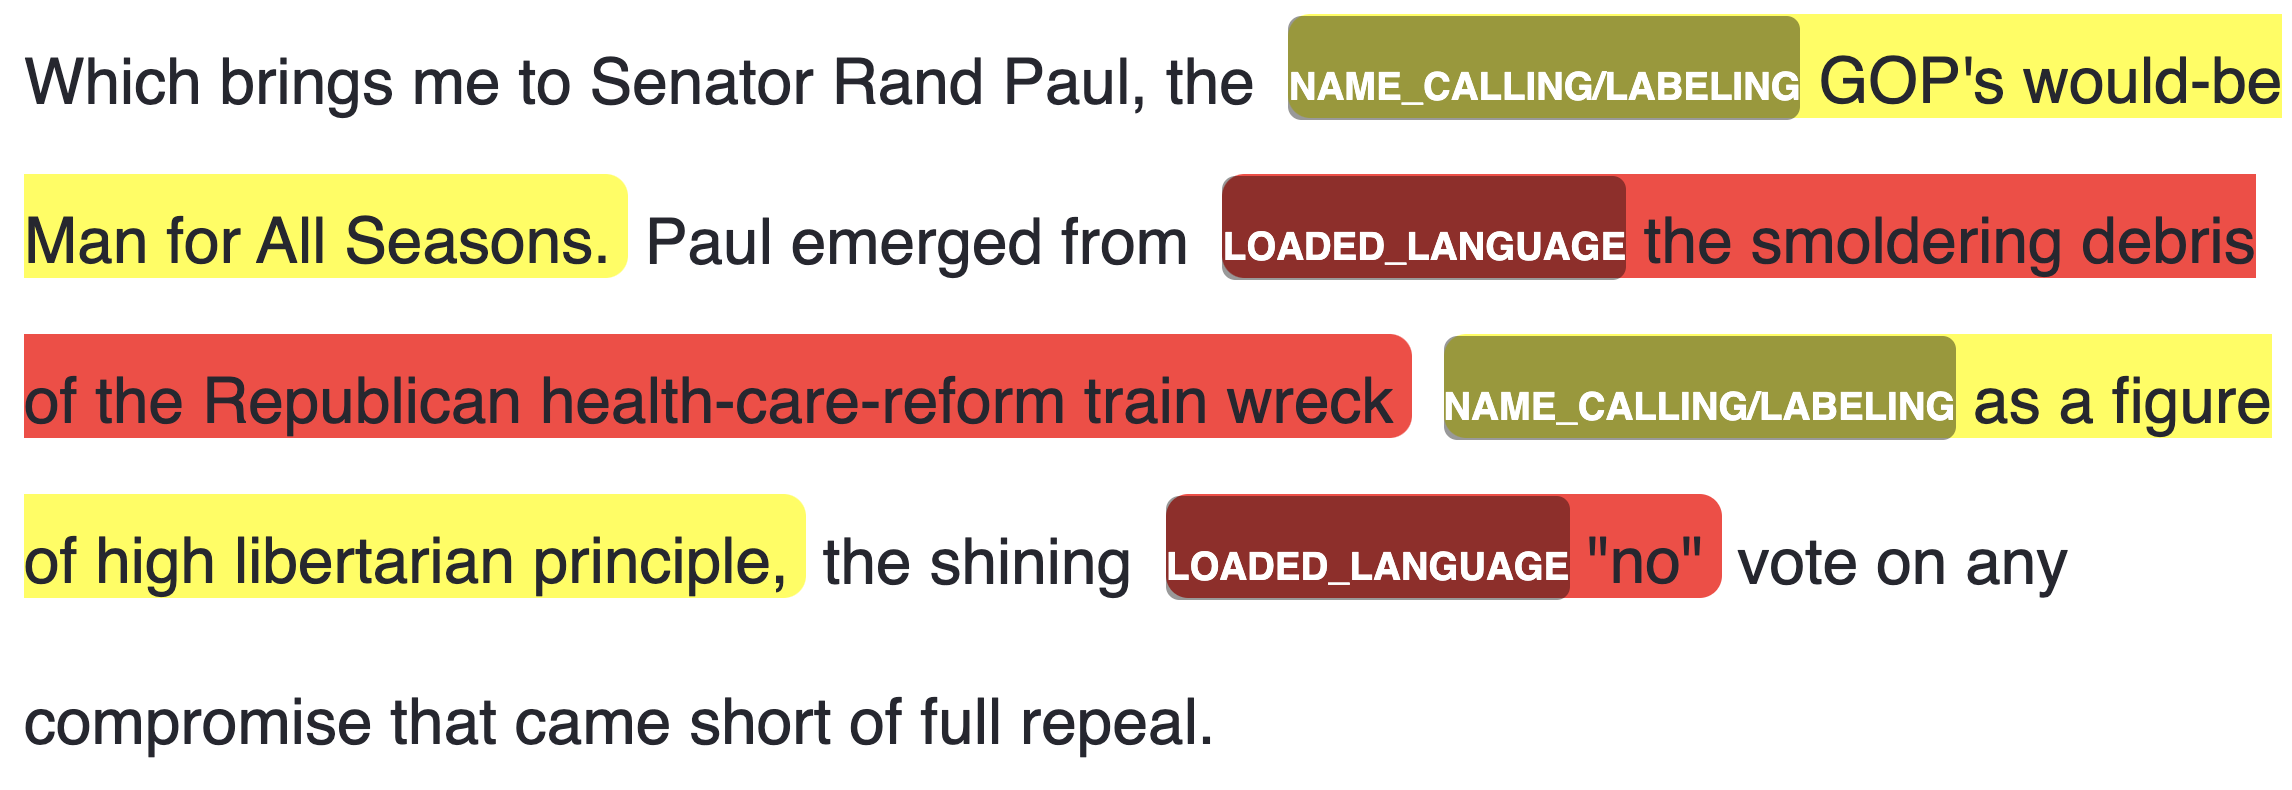
\includegraphics[width=\linewidth]{figures/propaganda_example_1_color.png}
    \caption{Detection of propaganda techniques using~\citet{baly2020we}.% the article comes from NationalReview, a source with Right-leaning bias.
    }
    \label{fig:propaganda_example_1}
\end{figure}


%For the propaganda analysis, we are focusing on the computational propaganda, defined as the propaganda that has been analysed by computational approaches. 
%The survey conducted by~\citet{da2020survey} displays the most important works, and also underlines the main limitation of current methods.
%The biggest limitation that we see, is that \emph{explainability is a desirable feature} but current approaches do not provide it.
%Most of the models only classify full articles as being propagandist or not~\cite{barron2019proppy,rashkin2017truth}, and this does not help to understand why.
%Therefore, another work focuses on fine-grained techniques~\cite{da2019fine}: every article analysed is annotated with labels coming from 18 different techniques, also indicating the spans affected by the techniques. So we can see where propaganda is inside an article and which specific techniques were used. Figure~\ref{fig:propaganda_example_1}

TODO: The datasets for detection: article-level, fine-grained

\subsubsection{Layers of information}
\label{ssec:lit_layers_of_info}

Talk here about different layers: 1 facts, 2 persuasion ( propaganda/argumentation/sentiment). Or in other terms: topical and non-topical elements.
These two elements can be expressed in different words, e.g. name+adjective, where the name is the topical element while the adjective can express the opinion of the writer (commenting, denigrating, complimenting, subjective).
Or they can also be expressed in the same word together: this is where word selection applies. For example, when the writer needs to find a word for communicating a certain concept ``?", they can choose whether to use X or Y. While these two words have the same underlying concept, they express it quite differently.

Propaganda: Communication with the goal to persuade

Hypothesis: we can observe the two layers distinctly?

\section{Political Leaning}
\label{sec:lit_leaning}

TODO: definition

Not going into political sciences. Here we take the definition L/R from mainly US context (democrats vs republicans) because most of the resources about news use it.

\subsection{Political Spectrum}

Comparing different scales:
- left/right
- moderate/extreme

\subsection{Political Leaning Classification}
\label{ssec:lit_leaning_classification}

FROM TTO2020

%First we present literature on political leaning prediction, then on propaganda detection, and how the two analyses could be connected. %with the possible points of contact and why the two analysis could benefit from an integration.

%\subsection{Political Leaning}
% Political leaning classification

Political leaning detection models have been produced for general media sources~\cite{budak} or for 
specific political corpora such as congressional records~\cite{gentzkow}, political party websites~\cite{yan2017perils}, and political blogs~\cite{ahmed201}.  
Others focused on inferring the political leaning of Twitter accounts~\cite{Cohen2013ClassifyingPO}, Facebook users~\cite{Bakshy1130}, politicians~\cite{thomas-etal-2006-get}, or political writers~\cite{iyyer-etal-2014-political}. 
Various analysis methods were used in such studies, such as linguistic analysis \cite{gentzkow}, graph analysis \cite{chen2017opinion}, topic modelling \cite{ahmed201, Cohen2013ClassifyingPO}, support vector machines (SVM) \cite{Bakshy1130,thomas-etal-2006-get}, and neural networks \cite{iyyer-etal-2014-political,baly2020we}. In this paper, we focus on detecting political learning of articles in a corpus of general news from a wide variety of sources (see Section~\ref{sec:dataset}), using a neural network approach fused with propaganda features. %\todo{description ok?} 

%often used supervised or unsupervised models applied to , or on opinion graph mining ~\cite{thomas-etal-2006-get}.

%gentzkow - linguistic analysis 
%yan2017perils - regression models and neural networks
%budak - supervised learning and crowdsourcing
%ahmed - topic models
%Cohen2013ClassifyingPO - SVM and topic models
%bakshy support vector machine 
%thomas - svm
%iyyer - NN
%chen - SVM, LDA

%Most models use supervised or unsupervised machine learning algorithms, trained using source annotations or crowdsourced articles annotations  
 
%underlined that most of the approaches do not generalise well across domains. 
%As~\citet{yan2017perils} underline, three different classifiers trained on different types of texts (domains: congressional records~\cite{gentzkow}, political websites, wiki) result in lack of cross-domain generalisability (classifier trained on different domain struggles to find correct label on another domain, and mixing the training data reduces performance confusing the models).

In~\citet{baly2020we}, authors used a BERT-based model for predicting the political leaning of individual articles. The model takes as input the text of the article and produces one of three labels: Left/Centre/Right. The model is trained with a corpus from AllSides website\footnote{\url{https://www.allsides.com}} which groups articles %with their political leaning 
according to the leaning of their source or of their author. %\todo{manually?}
%Authors found that 3.11\% of their 34737 articles from AllSides has a different leaning to that given to their sources (AllSides confirmed that this is due to using author-based leaning). 
%   \item source-level annotation: in most of the cases, the articles are annotated with the bias of the media outlet
 %   \item author-level annotation: sometimes, the articles are annotated with the bias of the specific writer, which can be
 % Similarly to \citet{baly2020we}, in this paper we also focus on classifying articles, regardless of their source and authorship. However, %unlike ~\cite{baly2020we}, 
 % unlike previous work, we use propaganda features in the political learning prediction model.   

% - Problem: learning the source instead of the political leaning
%Main focus in~\citet{baly2020we} is to classify individual articles regardless of the source or author. This generalises better with unseen sources, and with cases were there is a difference between the political leaning of a particular article from that of its source. Authors found that 3.11\% of their 34737 articles from AllSides has a different leaning to the given to their sources (AllSides confirmed that this is due to using author-based leaning labels for some articles). 


%Other approaches focus on learning the media bias of a the source~\cite{baly2020written,biessmann2016automating}.
%This is based on the observation that in their dataset (collected from AllSides) there are some articles (1,080 individual articles, 3.11\% on a total of 34737) having a leaning different from their source leaning.

%To clarify this point, we personally asked to the AllSides team about this discrepancy between article-level bias and source bias, and we understood that there are two types of annotation:
%\begin{itemize}
 %   \item source-level annotation: in most of the cases, the articles are annotated with the bias of the media outlet
 %   \item author-level annotation: sometimes, the articles are annotated with the bias of the specific writer, which can be different from the media bias\footnote{\url{https://www.allsides.com/media-bias/media-bias-ratings\#ratings}}
%\end{itemize}

%Therefore the 3.11\% is due to the author-level annotation. We want to underline that in this way, the annotation of the political leaning is not specifically assigned to the single article but instead it is assigned to the author. It is still a "distant supervision" in some extent.

% - Problem: domain generalisation does not work
%Other works on political orientation prediction underlined that most of the approaches do not generalise well across domains. As~\citet{yan2017perils} underline, three different classifiers trained on different types of texts (domains: congressional records, media websites, wiki) result in lack of cross-domain generalisability (classifier trained on different domain struggles to find correct label on another domain, and mixing the training data reduces performance confusing the models).


% TODO: Is this really a consequence of the previous paragraph?
%Because of this lack of generalisability, 
%Other models focused on identifying political leaning using opinion graphs that represent how (positive/neutral/negative) the political leaning sees a set of extracted entities~\cite{chen2017opinion}. The prediction of the classifier, after extracting the entities in the text, compares the orientation towards the entities and picks the most similar side.
%The task of topical stance is also explored in other works in relationship to the political leaning of a whole news source~\cite{stefanov2020predicting}.
%A similar approach is described in~\citet{jiang2008political}, where instead of opinion the term used is subjectivities. The authors show how, by using the same model (Bag of Words) on the subjective sentences only, it is actually easier to classify political leaning. Furthermore, they mine Opinion Expressions which represent the orientation towards specific expressions (e.g., the liberal political leaning usually refers to ``democratic party'' using a positive subjectivity).
%These models rely on the fact that political leanings often have a stable view on some topics\footnote{\url{https://en.wikipedia.org/wiki/Right-wing_politics}}\footnote{\url{https://en.wikipedia.org/wiki/Left-wing_politics}}.








% Sentiment analysis

% Propaganda analysis

% Fine-grained

% AllSides and comparison of multiple sides, the summary contains some insights about the biggest differences between the political sides.

% Bias / political leaning classifier:
% - baly et al 2020: just based on text
% - we could help the models focusing on the layer of presentation/bias/propaganda instead of having the full text



% Two axes:
% - common/unique
% - objective/subjective/framing

% Different. The first one can be observed with similarity analysis. The second one with sentiment/propaganda/framing analysis.

% The left/center/right political leaning is mostly positioned on the common/unique axis.

% Hypothesis: the two axes are very much correlated. Looking at the framing axis can help to distinguish political bias.

% We try in the next sections to see if this is true.



\section{Similarity between articles}
\label{sec:lit_relationships}

?? Is this necessary? Or just mention corroboration/omission in framing techniques?

\section{Other related phenomena}

TODO: here talk about misinformation, argumentation mining and defend the scope of this thesis: propaganda.

But at the same time mention the relationship with them

\subsection{Propaganda and Misinformation}

Work of~\citet{orrumachine} where persuasiveness is observed to exist more in fake news outlets: discursive repertoires that are more persuasive appear more in fake, while some other discursive repertoires that are less persuasive appear in more trustworthy news outlets.




\cite{roozenbeek2022countering} Good evidence that making people aware is helpful, people can learn to recognise manipulation techniques (it worked on YouTube). The paper talks about manipulation, but the techniques overlap with propaganda and logical fallacies. Also shifts the goal from recognising True/False to recognising manipulation. Work from Psychology.

Cite TTO2019 comparison of different credibility measures, and we saw that propagandistic sources are usually considered as part of misinformation (MBFC dataset).


\cite{romain2022misinformation} persuasive writing strategies for misinformation detection (TODO analyse this paper)

\subsubsection{Rating news sources in different aspects}

TODO: here talk about all the tools/websites that rank news sources or score them with respect to misinformation/propaganda/bias/leaning

\subsection{Propaganda and Populism}

Relationship between propaganda and populism:
~\cite{tumber2021routledge,pasquino2008populism}
%https://ebrary.net/177441/sociology/the_routledge_companion_to_media_disinformation_and_populism
they are very strictly linked
% http://www.ask-force.org/web/Fundamentalists/Pasquino-Populism-and-Democrady-2005.pdf 


Literature shows “populism” as a concept together with Propaganda
What is the difference between populism and propaganda?
Can we use some datasets about populism to understand how they contain propaganda?

Dataset found: populism in political speeches %https://dataverse.harvard.edu/dataset.xhtml?persistentId=doi:10.7910/DVN/LFTQEZ&version=2.0 
Each annotator (4 for each speech) gave a score between 0 (non-populistic) to 2 (very populistic)
4961 rows 
1240 deduped (352 left, 256 center, 469 right, 652 NA)
Languages: 265 en (304 es, 148 pt, …),
Leaning of the english ones: (36 left, 37 center, 84 right, 106 NA)


\subsection{Opinion and Subjectivity and Manipulation?}

\section{Scope of this work}

Main ingredients:
- Propaganda detection
- Political leaning

We see that the two can be related and we want to understand their relationships.
How does propaganda change across political leaning?
Can we recognise the political orientation of a piece of news from how it uses propaganda techniques?
How does propaganda relate to shared/unique information? How do small variations relate to propaganda?
